\documentclass[12pt]{article}
\usepackage[margin=2.5cm]{geometry}
\usepackage{enumerate}
\usepackage{amsfonts}
\usepackage{amsmath}
\usepackage{fancyhdr}
\usepackage{amsmath}
\usepackage{amssymb}
\usepackage{amsthm}
\usepackage{mdframed}
\usepackage{graphicx}
\usepackage{subcaption}
\usepackage{adjustbox}
\usepackage{listings}
\usepackage{xcolor}
\usepackage{booktabs}
\usepackage[utf]{kotex}

\definecolor{codegreen}{rgb}{0,0.6,0}
\definecolor{codegray}{rgb}{0.5,0.5,0.5}
\definecolor{codepurple}{rgb}{0.58,0,0.82}
\definecolor{backcolour}{rgb}{0.95,0.95,0.92}

\lstdefinestyle{mystyle}{
    backgroundcolor=\color{backcolour},
    commentstyle=\color{codegreen},
    keywordstyle=\color{magenta},
    numberstyle=\tiny\color{codegray},
    stringstyle=\color{codepurple},
    basicstyle=\ttfamily\footnotesize,
    breakatwhitespace=false,
    breaklines=true,
    captionpos=b,
    keepspaces=true,
    numbers=left,
    numbersep=5pt,
    showspaces=false,
    showstringspaces=false,
    showtabs=false,
    tabsize=1
}

\lstset{style=mystyle}

\begin{document}
\title{CSC236 Term Test 1 Version 2 Solution}
\author{Hyungmo Gu}
\maketitle

\section*{Question 1}
\begin{itemize}
    \item

    \begin{proof}
    Define $P(n):f(n) = 3^n$.

    \bigskip

    I will use complete induction to prove that $\forall n \in \mathbb{N}, n > 2 \Rightarrow \:P(n)$.

    \bigskip

    \underline{\textbf{Base Case ($n = 0$):}}

    \bigskip

    Let $n = 0$.

    \bigskip

    Then, the definition of $f(n)$ tells us $f(n) = 1$.

    \bigskip

    Then, we have

    \begin{align}
        f(n) &= 3^0\\
        &= 3^n
    \end{align}

    \bigskip

    Thus, $P(n)$ follows.

    \bigskip

    \underline{\textbf{Base Case ($n = 1$):}}

    \bigskip

    Let $n = 1$.

    \bigskip

    Then, the definition of $f(n)$ tells us $f(n) = 3$.

    \bigskip

    Then, we have

    \begin{align}
        f(n) &= 3^1\\
        &= 3^n
    \end{align}

    \bigskip

    Thus, $P(n)$ follows.

    \bigskip

    \underline{\textbf{Base Case ($n = 2$):}}

    \bigskip

    Let $n = 2$.

    \bigskip

    Then, the definition of $f(n)$ tells us $f(n) = 9$.

    \bigskip

    Then, we have

    \begin{align}
        f(n) &= 3^2\\
        &= 3^n
    \end{align}

    \bigskip

    Thus, $P(n)$ follows.

    \bigskip

    \underline{\textbf{Case ($n > 2$):}}

    \bigskip

    Assume $n > 2$.

    \bigskip

    Then, since $0 \leq n - 1 < n$, $0 \leq n -2 < n$, and $0 \leq n - 3 < n$,
    the complete induction tells us $P(n-1)$, $P(n-2)$, and $P(n-3)$, i.e.
    $f(n-1) = 3^{n-1}$, $f(n-2) = 3^{n-2}$, and $f(n-3) = 3^{n-3}$, respectively.

    \bigskip

    Then, using these facts, we can write

    \begin{align}
        f(n) &= f(n-1) + 3f(n-2) + 9f(n-3)\\
        &= 3^{n-1} + 3 \cdot 3^{n-2} + 3^2 \cdot 3^{n-3}\\
        &= 3^{n-1} + 3^{n-1} + 3^{n-1}\\
        &= 3^{n-1}(1 + 1 + 1)\\
        &= 3^{n-1}3\\
        &= 3^n
    \end{align}

    \bigskip

    Thus, $P(n)$ follows.
    \end{proof}
\end{itemize}

% \bigskip

% \begin{mdframed}
%     \underline{\textbf{Rough Work:}}

%     \bigskip

%     Define $P(n):f(n) = 3^n$.

%     \bigskip

%     I will use complete induction to prove that $\forall n \in \mathbb{N}, n > 2 \Rightarrow \:P(n)$.

%     \begin{enumerate}[1.]
%         \item Inductive Step

%         \begin{mdframed}
%         \underline{\textbf{Inductive Step:}}

%         \bigskip

%         Let $n \in \mathbb{N}$. Assume $n > 2$. Assume
%         $H(n):\bigwedge\limits_{i=0}^{n-1} P(i)$. I will prove $P(n)$ follows.
%         That is, $f(n) = 3^n$.
%         \end{mdframed}

%         \item Base Case ($n = 0$)

%         \begin{mdframed}
%         \underline{\textbf{Base Case ($n = 0$):}}

%         \bigskip

%         Let $n = 0$.

%         \bigskip

%         Then, the definition of $f(n)$ tells us $f(n) = 1$.

%         \bigskip

%         Then, we have

%         \begin{align}
%             f(n) &= 3^0\\
%             &= 3^n
%         \end{align}

%         \bigskip

%         Thus, $P(n)$ follows.
%         \end{mdframed}

%         \item Base Case ($n = 1$)

%         \begin{mdframed}
%         \underline{\textbf{Base Case ($n = 1$):}}

%         \bigskip

%         Let $n = 1$.

%         \bigskip

%         Then, the definition of $f(n)$ tells us $f(n) = 3$.

%         \bigskip

%         Then, we have

%         \begin{align}
%             f(n) &= 3^1\\
%             &= 3^n
%         \end{align}

%         \bigskip

%         Thus, $P(n)$ follows.

%         \end{mdframed}

%         \item Base Case ($n = 2$)

%         \begin{mdframed}
%         \underline{\textbf{Base Case ($n = 2$):}}

%         \bigskip

%         Let $n = 2$.

%         \bigskip

%         Then, the definition of $f(n)$ tells us $f(n) = 9$.

%         \bigskip

%         Then, we have

%         \begin{align}
%             f(n) &= 3^2\\
%             &= 3^n
%         \end{align}

%         \bigskip

%         Thus, $P(n)$ follows.

%         \end{mdframed}

%         \item Case ($n > 2$)

%         \begin{mdframed}
%         \underline{\textbf{Case ($n > 2$):}}

%         \bigskip

%         Assume $n > 2$.

%         \bigskip

%         Then, since $0 \leq n - 1 < n$, $0 \leq n -2 < n$, and $0 \leq n - 3 < n$,
%         the complete induction tells us $P(n-1)$, $P(n-2)$, and $P(n-3)$, i.e.
%         $f(n-1) = 3^{n-1}$, $f(n-2) = 3^{n-2}$, and $f(n-3) = 3^{n-3}$, respectively.

%         \bigskip

%         Then, using these facts, we can write

%         \begin{align}
%             f(n) &= f(n-1) + 3f(n-2) + 9f(n-3)\\
%             &= 3^{n-1} + 3 \cdot 3^{n-2} + 3^2 \cdot 3^{n-3}\\
%             &= 3^{n-1} + 3^{n-1} + 3^{n-1}\\
%             &= 3^{n-1}(1 + 1 + 1)\\
%             &= 3^{n-1}3\\
%             &= 3^n
%         \end{align}

%         \bigskip

%         Thus, $P(n)$ follows.
%         \end{mdframed}
%     \end{enumerate}

% \end{mdframed}

\bigskip

\begin{mdframed}
    \underline{\textbf{Correct Solution:}}

    \bigskip

    Define $P(n):f(n) = 3^n$.

    \bigskip

    I will use complete induction to prove that \color{red}$\forall n \in \mathbb{N}, \:P(n)$\color{black}.

    \bigskip

    \color{red}
    \underline{\textbf{Inductive Step:}}

    \bigskip

    Let $n \in \mathbb{N}$. Assume $H(n):\bigwedge\limits_{i=0}^{n-1} P(i)$. I will prove $P(n)$ follows.
    That is, $f(n) = 3^n$.
    \color{black}

    \bigskip

    \underline{\textbf{Base Case ($n = 0$):}}

    \bigskip

    Let $n = 0$.

    \bigskip

    Then, the definition of $f(n)$ tells us $f(n) = 1$.

    \bigskip

    Then, we have

    \begin{align}
        f(n) &= 3^0\\
        &= 3^n
    \end{align}

    \bigskip

    Thus, $P(n)$ follows.

    \bigskip

    \underline{\textbf{Base Case ($n = 1$):}}

    \bigskip

    Let $n = 1$.

    \bigskip

    Then, the definition of $f(n)$ tells us $f(n) = 3$.

    \bigskip

    Then, we have

    \begin{align}
        f(n) &= 3^1\\
        &= 3^n
    \end{align}

    \bigskip

    Thus, $P(n)$ follows.

    \bigskip

    \underline{\textbf{Base Case ($n = 2$):}}

    \bigskip

    Let $n = 2$.

    \bigskip

    Then, the definition of $f(n)$ tells us $f(n) = 9$.

    \bigskip

    Then, we have

    \begin{align}
        f(n) &= 3^2\\
        &= 3^n
    \end{align}

    \bigskip

    Thus, $P(n)$ follows.

    \bigskip

    \underline{\textbf{Case ($n > 2$):}}

    \bigskip

    Assume $n > 2$.

    \bigskip

    Then, since $0 \leq n - 1 < n$, $0 \leq n -2 < n$, and $0 \leq n - 3 < n$,
    the complete induction tells us $P(n-1)$, $P(n-2)$, and $P(n-3)$, i.e.
    $f(n-1) = 3^{n-1}$, $f(n-2) = 3^{n-2}$, and $f(n-3) = 3^{n-3}$, respectively.

    \bigskip

    Then, using these facts, we can write

    \begin{align}
        f(n) &= f(n-1) + 3f(n-2) + 9f(n-3) & \color{red}[\text{By definition, since $n > 2$}]\color{black}\\
        &= 3^{n-1} + 3 \cdot 3^{n-2} + 3^2 \cdot 3^{n-3}\\
        &= 3^{n-1} + 3^{n-1} + 3^{n-1}\\
        &= 3^{n-1}(1 + 1 + 1)\\
        &= 3^{n-1}3\\
        &= 3^n
    \end{align}

    \bigskip

    Thus, $P(n)$ follows.
    \bigskip
\end{mdframed}

\bigskip

\underline{\textbf{Notes:}}

\bigskip

\begin{enumerate}[1.]
    \item Learned that $n > i$ in $\forall n \in \mathbb{N}, n > i \Rightarrow \:P(n)$
    is used when $P(n)$ is true starting $i + 1$.

    \bigskip

    If $P(n)$ is true for all natural numbers, then $\forall n \in \mathbb{N}, P(n)$
    is used.

    \item Learned that `Assume $n > 2$' in `Let $n \in \mathbb{N}$. Assume $n > 2$.
    Assume $H(n):\bigwedge\limits_{i=0}^{n-1} P(i)$'. is used
    when $P(i)$ is true starting $n = 3$.

    \bigskip

    If $P(i)$ is true for all natural numbers, then, `Let $n \in \mathbb{N}$. Assume
    $H(n):\bigwedge\limits_{i=0}^{n-1} P(i)$' is used.

\end{enumerate}

\section*{Question 2}

\begin{itemize}
    \item

    Given the statement to prove

    \begin{center}
        $P(x,y,z,w):$ There are no positive integers $x,y,z,w$ such that $x^4 + 3y^4 + 9z^4 = 27w^4$.
    \end{center}

    \bigskip

    \begin{proof}
    I will prove $P(x,y,z,w)$ using proof by contradiction.

    \bigskip

    Assume $\exists x,y,z,w \in \mathbb{N}^+$, $x^4 + 3y^4 + 9z^4 = 27w^4$.

    \bigskip

    Then, the set $X = \{x \in \mathbb{N}^+ \mid \exists y,z,w \in \mathbb{N}^+, x^4 + 3y^4 + 9z^4 = 27w^4\}$ is
    not empty.

    \bigskip

    Then, by principle of well-ordering, there is smallest positive integer
    $x_0 \in X$, and postive integers $y_0,z_0,w_0 \in \mathbb{N}^+$ such
    that $x_0^4 + 3y_0^4 + 9z_0^4 = 27w_0^4$.

    \bigskip

    Then,
    \setcounter{equation}{0}
    \begin{align}
        \begin{split}
        x_0^4 + 3y_0^4 + 9z_0^4 = 27w_0^4 &\Rightarrow x_0^4 = 27w_0^4 - 3y_0^4 - 9z_0^4\\
        & \Rightarrow 3 \mid x_0^4 \Rightarrow 3 \mid x_0
        \end{split} & [\text{By hint}]\\[1em]
        \begin{split}
        \text{Let $\exists x_1 \in \mathbb{N}^+$, $x_0 = 3x_1$} &\Rightarrow x_0^4 + 3y_0^4 + 9z_0^4 = 27w_0^4\\
        &\Rightarrow 3y_0^4 = 27w_0^4 - 9z_0^4 - x_0^4\\
        &\Rightarrow 3y_0^4 = 27w_0^4 - 9z_0^4 - 3^4x_1^4\\
        &\Rightarrow y_0^4 = 9w_0^4 - 3z_0^4 - 3^3x_1^4\\
        &\Rightarrow 3 \mid y_0^4 \Rightarrow 3 \mid y_0
        \end{split} & [\text{By hint}]\\[1em]
        \begin{split}
        \text{Let $\exists y_1 \in \mathbb{N}^+$, $y_0 = 3y_1$} &\Rightarrow x_0^4 + 3y_0^4 + 9z_0^4 = 27w_0^4\\
        &\Rightarrow 9z_0^4 = 27w_0^4 - 3y_0^4 - x_0^4\\
        &\Rightarrow 9z_0^4 = 27w_0^4 - 3^5y_1^4 - 3^4x_1^4\\
        &\Rightarrow z_0^4 = 3w_0^4 - 3^3y_1^4 - 3^2x_1^4\\
        &\Rightarrow 3 \mid z_0^4 \Rightarrow 3 \mid z_0
        \end{split} & [\text{By hint}]\\[1em]
        \begin{split}
        \text{Let $\exists w_1 \in \mathbb{N}^+$, $w_0 = 3w_1$} &\Rightarrow x_0^4 + 3y_0^4 + 9z_0^4 = 27w_0^4\\
        &\Rightarrow 3^4x_1^4 + 3^5y_1^4 + 3^6z_1^4 = 3^7w_1^4\\
        &\Rightarrow x_1^4 + 3y_1^4 + 3^2z_1^4 = 3^3w_1^4\\
        &\Rightarrow x_1^4 + 3y_1^4 + 9z_1^4 = 27w_1^4\\
        &\Rightarrow x_1 \in X
        \end{split}
    \end{align}

    \bigskip

    Then, this leads to contradiction, because we know $x_1 < x_0$, $x_1 \in X$,
    but $x_0$ is the smallest number in $X$.

    \bigskip

    Thus, we can conclude the assumption is false.

    \end{proof}
\end{itemize}

\bigskip

\begin{mdframed}
    \underline{\textbf{Correct Solution:}}

    \bigskip

    Given the statement to prove

    \begin{center}
        $P(x,y,z,w):$ There are no positive integers $x,y,z,w$ such that $x^4 + 3y^4 + 9z^4 = 27w^4$.
    \end{center}

    \bigskip

    \begin{proof}
    I will prove $P(x,y,z,w)$ using proof by contradiction.

    \bigskip

    Assume $\exists x,y,z,w \in \mathbb{N}^+$, $x^4 + 3y^4 + 9z^4 = 27w^4$.

    \bigskip

    Then, the set $X = \{x \in \mathbb{N}^+ \mid \exists y,z,w \in \mathbb{N}^+, x^4 + 3y^4 + 9z^4 = 27w^4\}$ is
    not empty.

    \bigskip

    Then, \color{red}since $X$ is subset of $\mathbb{N}$\color{black}, by
    principle of well-ordering, there is smallest positive integer $x_0 \in X$.
    \color{red}Furthermore\color{black}, there are postive integers
    $y_0,z_0,w_0 \in \mathbb{N}^+$ such that $x_0^4 + 3y_0^4 + 9z_0^4 = 27w_0^4$.

    \bigskip

    Then,
    \setcounter{equation}{0}
    \begin{align}
        \begin{split}
        x_0^4 + 3y_0^4 + 9z_0^4 = 27w_0^4 &\Rightarrow x_0^4 = 27w_0^4 - 3y_0^4 - 9z_0^4\\
        & \Rightarrow 3 \mid x_0^4 \Rightarrow 3 \mid x_0
        \end{split} & [\text{By hint}]\\[1em]
        \begin{split}
        \text{Let $\exists x_1 \in \mathbb{N}^+$, $x_0 = 3x_1$} &\Rightarrow x_0^4 + 3y_0^4 + 9z_0^4 = 27w_0^4\\
        &\Rightarrow 3y_0^4 = 27w_0^4 - 9z_0^4 - x_0^4\\
        &\Rightarrow 3y_0^4 = 27w_0^4 - 9z_0^4 - 3^4x_1^4\\
        &\Rightarrow y_0^4 = 9w_0^4 - 3z_0^4 - 3^3x_1^4\\
        &\Rightarrow 3 \mid y_0^4 \Rightarrow 3 \mid y_0
        \end{split} & [\text{By hint}]\\[1em]
        \begin{split}
        \text{Let $\exists y_1 \in \mathbb{N}^+$, $y_0 = 3y_1$} &\Rightarrow x_0^4 + 3y_0^4 + 9z_0^4 = 27w_0^4\\
        &\Rightarrow 9z_0^4 = 27w_0^4 - 3y_0^4 - x_0^4\\
        &\Rightarrow 9z_0^4 = 27w_0^4 - 3^5y_1^4 - 3^4x_1^4\\
        &\Rightarrow z_0^4 = 3w_0^4 - 3^3y_1^4 - 3^2x_1^4\\
        &\Rightarrow 3 \mid z_0^4 \Rightarrow 3 \mid z_0
        \end{split} & [\text{By hint}]\\[1em]
        \begin{split}
        \text{Let $\exists w_1 \in \mathbb{N}^+$, $w_0 = 3w_1$} &\Rightarrow x_0^4 + 3y_0^4 + 9z_0^4 = 27w_0^4\\
        &\Rightarrow 3^4x_1^4 + 3^5y_1^4 + 3^6z_1^4 = 3^7w_1^4\\
        &\Rightarrow x_1^4 + 3y_1^4 + 3^2z_1^4 = 3^3w_1^4\\
        &\Rightarrow x_1^4 + 3y_1^4 + 9z_1^4 = 27w_1^4\\
        &\Rightarrow x_1 \in X
        \end{split}
    \end{align}

    \bigskip

    Then, this leads to contradiction, because we know $x_1 < x_0$, $x_1 \in X$,
    but $x_0$ is the smallest number in $X$.

    \bigskip

    Thus, we can conclude the assumption is false.

    \end{proof}

\end{mdframed}

\bigskip

\underline{\textbf{Note:}}

\bigskip

\begin{itemize}
    \item Noticed professor wrote `Divide by 3' as a reasoning in calculation.

    \begin{center}
    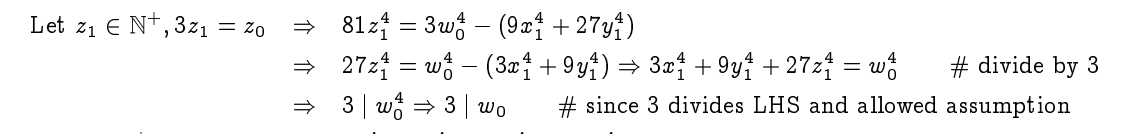
\includegraphics[width=0.8\linewidth]{images/term_test_1_v2_q2_note.png}
    \end{center}
\end{itemize}

% \bigskip

% \begin{mdframed}
%     \underline{\textbf{Rough Work:}}

%     \bigskip

%     Given the statement to prove

%     \begin{center}
%         $P(x,y,z,w):$ There are no positive integers $x,y,z,w$ such that $x^4 + 3y^4 + 9z^4 = 27w^4$.
%     \end{center}

%     \bigskip

%     I will prove $P(x,y,z,w)$ using proof by contradiction.

%     \bigskip

%     Assume $\exists x,y,z,w \in \mathbb{N}^+$, $x^4 + 3y^4 + 9z^4 = 27w^4$.

%     \begin{enumerate}[1.]
%         \item Show that the set $X = \{x \in \mathbb{N}^+ \mid \exists y,z,w \in \mathbb{N}^+, x^4 + 3y^4 + 9z^4 = 27w^4\}$

%         \begin{mdframed}
%         Then, the set $X = \{x \in \mathbb{N}^+ \mid \exists y,z,w \in \mathbb{N}^+, x^4 + 3y^4 + 9z^4 = 27w^4\}$ is
%         not empty.
%         \end{mdframed}

%         \item Show there is smallest positive integer $x_0 \in X$ and positive integers $y_0,z_0,w_0 \in \mathbb{N}^+$,
%         such that $x_0^4 + 3y_0^4 + 9z_0^4 = 27w_0^4$ using principle of well-ordering

%         \begin{mdframed}
%         Then, by principle of well-ordering, there is smallest positive integer
%         $x_0 \in X$, and postive integers $y_0,z_0,w_0 \in \mathbb{N}^+$ such
%         that $x_0^4 + 3y_0^4 + 9z_0^4 = 27w_0^4$.

%         \end{mdframed}

%         \item Show there is $x_1 < x_0$ and $x_1 \in X$

%         \begin{mdframed}
%         Then,
%         \setcounter{equation}{0}
%         \begin{align}
%             \begin{split}
%             x_0^4 + 3y_0^4 + 9z_0^4 = 27w_0^4 &\Rightarrow x_0^4 = 27w_0^4 - 3y_0^4 - 9z_0^4\\
%             & \Rightarrow 3 \mid x_0^4 \Rightarrow 3 \mid x_0
%             \end{split} & [\text{By hint}]\\[1em]
%             \begin{split}
%             \text{Let $\exists x_1 \in \mathbb{N}^+$, $x_0 = 3x_1$} &\Rightarrow x_0^4 + 3y_0^4 + 9z_0^4 = 27w_0^4\\
%             &\Rightarrow 3y_0^4 = 27w_0^4 - 9z_0^4 - x_0^4\\
%             &\Rightarrow 3y_0^4 = 27w_0^4 - 9z_0^4 - 3^4x_1^4\\
%             &\Rightarrow y_0^4 = 9w_0^4 - 3z_0^4 - 3^3x_1^4\\
%             &\Rightarrow 3 \mid y_0^4 \Rightarrow 3 \mid y_0
%             \end{split} & [\text{By hint}]\\[1em]
%             \begin{split}
%             \text{Let $\exists y_1 \in \mathbb{N}^+$, $y_0 = 3y_1$} &\Rightarrow x_0^4 + 3y_0^4 + 9z_0^4 = 27w_0^4\\
%             &\Rightarrow 9z_0^4 = 27w_0^4 - 3y_0^4 - x_0^4\\
%             &\Rightarrow 9z_0^4 = 27w_0^4 - 3^5y_1^4 - 3^4x_1^4\\
%             &\Rightarrow z_0^4 = 3w_0^4 - 3^3y_1^4 - 3^2x_1^4\\
%             &\Rightarrow 3 \mid z_0^4 \Rightarrow 3 \mid z_0
%             \end{split} & [\text{By hint}]\\[1em]
%             \begin{split}
%             \text{Let $\exists w_1 \in \mathbb{N}^+$, $w_0 = 3w_1$} &\Rightarrow x_0^4 + 3y_0^4 + 9z_0^4 = 27w_0^4\\
%             &\Rightarrow 3^4x_1^4 + 3^5y_1^4 + 3^6z_1^4 = 3^7w_1^4\\
%             &\Rightarrow x_1^4 + 3y_1^4 + 3^2z_1^4 = 3^3w_1^4\\
%             &\Rightarrow x_1^4 + 3y_1^4 + 9z_1^4 = 27w_1^4\\
%             &\Rightarrow x_1 \in X
%             \end{split}
%         \end{align}

%         \end{mdframed}

%         \item Conclude proof by contradiction

%         \begin{mdframed}
%         Then, this leads to contradiction, because we know $x_1 < x_0$, $x_1 \in X$,
%         but $x_0$ is the smallest number in $X$.

%         \bigskip

%         Thus, we can conclude the assumption is false.
%         \end{mdframed}
%     \end{enumerate}
% \end{mdframed}

\section*{Question 3}

\end{document}